\paragraph{Principal Component Analysis}
\subparagraph{Intuitive}
PCA can be thought of as \tB{fitting a $p-dimensional$ to the data, which each axis of the
ellipsoid represents a principal component}. If some axis of the ellipsoid is small, then the
variance along that axis is also small, and by omitting that axis and its corresponding principal
component from our representation of the dataset. 

\subparagraph{Methods}
To find the axes ellipsoid, we must first subtract the mean of each variable from the dataset
to center the data around the origin. 
\begin{enumerate}
	\item \sB{Subtract the mean of each variable} from the dataset to center the data around 
		the origin.
	\item \sB{Computing the covariance matrix} of the data and \sB{calculate the eigenvalues} and
		corresponding eigenvectors.
	\item \sB{Normalize each of the orthogonal eigenvectors} to turn into unit vectors.
\end{enumerate}
Then each of the mutually orthogonal, unit eigenvectors can be interpreted as an axis of the 
ellipsoid fitted to the data.\\ Our covariance matrix will be transformed into a diagonalised
form with the diagonal elements representing the variance of each axis.\\
The proportion of the variance that each eigenvector represents can be calculated by dividing 
the eigenvalue corresponding to that eigenvector by the sum of all eigenvalues.

\subparagraph{Mathematically}
PCA is defined as an orthogonal linear transformation that transforms the data to a new
coordinate system such that the greatest variance by some scalar projection of the 
data comes to lie on the first coordinate (the first principal component), the second greatest
variance on the second coordinate.\\

The transformation is defined by a \sB{set of size $l$ of $p-dimensional$ vectors of weights}
$\bm{\omega}_{(k)}=(\omega_{1},\cdots,\omega_{p})_{(k)}$, with $k\in\inter{1}{l}$, \sB{that map each
row vector} $\bm{x}_{(i)}$ of $\bm{X}$ \sB{to a new vector of principal component scores} $t_{(i)}=
(t_{1}, \cdots, t_{l})_{(i)}$ given by:
$\forall(i,k)\in\inter{1}{n}\times\inter{1}{l}{t_{k}}_{(i)}=\sP{\bm{x}_{i}}{\bm{\omega}_{(k)}}
\text{ with }l\leq p$\\

\tB{In order to maximize variance}, the first weight vector $\bm{\omega}_{(1)}$ thus has to satisfy:
\begin{center}
$\bm{\omega}_{(1)} = \max\limits_{\norm{\bm{\omega}}=1}\norm{\bm{X}\bm{\omega}}^{2}=
\max\limits_{\norm{\bm{\omega}}=1}\left(\bm{X}\bm{\omega}\right)^{T}\bm{X}\bm{\omega}$
\end{center}
Since $\bm{\omega}_{(1)}$ has been defined to be a unit vector, it equivalently also satisfies:
\begin{center}
\enc{$\bm{\omega}_{(1)}=\max\limits_{\norm{\bm{\omega}}=1}\dfrac{\bm{\omega}^{T}\bm{X}^{T}\bm{X}\bm{
\omega}}{\bm{\omega}^{T}\bm{\omega}}$}
\end{center}
The quantity to be maximised can be recognized as a Rayleigh quotient. A standard result \sB{for a 
positive semidefinite matrix such as $\bm{X}^{T}\bm{X}$ is that the Rayleigh quotient's maximum
possible value is the largest eigenvalue of the matrix, which occurs when $\bm{\omega}$ is the 
corresponding eigenvector}.\\

\textbf{\emph{Further components}}:\\
The $k^{th}$ component can be found by subtracting the first $k-1$ principal components from
$\bm{X}$:
\tB{$\hat{\bm{X}}_{k}=\bm{X}-\su{{s=1}}{k-1}\bm{X}\bm{\omega}_{(s)}\bm{\omega}_{(s)}^{T}$}
and then finding the weight vector which extracts the maximum variance from this new data matrix:
\begin{center}
\encB{$\bm{\omega}_{(k)}=\max\limits_{\norm{\bm{\omega}}=1}\norm{\hat{\bm{X}}_{k}\bm{\omega}}^{2}=
\max\limits_{\norm{\bm{\omega}}=1}\dfrac{\bm{\omega}^{T}\hat{\bm{X}}_{k}^{T}\hat{\bm{X}}_{k}\bm{
\omega}} {\bm{\omega}^{T}\bm{\omega}}$}
\end{center}
It turns out that this gives the remaining eigenvectors of $\bm{X}^{T}\bm{X}$, with the maximum 
values for the quantity in brackets given by their corresponding eigenvalues. Thus the weight vectors
are eigenvectors of $\bm{X}\bm{X}^{T}$.\\
The \sR{full principal components decomposition of $\bm{X}$ can therefore be given as:
$\bm{T}=\bm{X\Omega}$}
where \tR{$\bm{\Omega}$ is a $p\times p$ of weights whose columns are the eigenvectors of 
$\bm{X}^{T}\bm{X}$}.

\begin{figure}[H]
	\begin{center}
		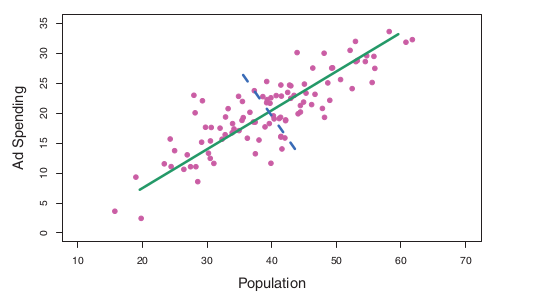
\includegraphics[width=\textwidth]{./chap/1chap/5sec/images/3principalCompoment.png} \end{center}
	\caption{The population size and ad spending for 100 different
	cities are shown as purple circles. The green solid line
	indicates the first principal component, and the blue dashed
	line indicates the second principal compoment.}
	\label{fig:3principalCompoment}
\end{figure}

\subparagraph{Principal Components Regression and Ridge Regression}
The \emph{Principal Components Regression} (PCR) approach \tB{involves
constructing the first $M$ principal components $\prth{Z}{i}{M}$
and then using these components as the predictors in a linear 
regression model that is fit using least squares}.\\

One can show that PCR and Ridge Regression are very closely related, 
one can even think of ridge regression as a continuous version of PCR.
\\
When performing PCR we generally recommend \emph{standardizing} each
predictor, using, prior to generating the principal components.\\

Ridge regression shrinks the coefficients of the principal components,
shrinking more depending on the size of the corresponding eigenvalue;
principal components regression discard the $p-M$ smallest eigenvalue
components.\\
\subparagraph{Python Code}
\begin{python}
import numpy as np
import pandas as pd
import matplotlib.pyplot as plt
import statsmodels.api as sm
from statsmodels.multivariate.pca import PCA
import sklearn
from sklearn.preprocessing import StandardScaler
from sklearn.decomposition import PCA as PCA_sk

df = pd.read_csv('myfile.csv', sep=';')
X, y = df.iloc[:, 1:], df.iloc[:, 0]
pca_model = PCA(X,
    standardize=False, # mean 0 and unit variance
    demean=True # to subtract columns by their mean
)
# Standardize the Data
fig = pca_model.plot_scree(log_scale=False) # to plot the explained
# variance of components.
print(pca_model.loadings.iloc[:, :2]).argsort() # to
# estimate the implication of a given variable in a the
# 2 first components.

# Computation
X_rm_mean = StandardScaler(with_std=False).fit_transform(X)
pca = PCA_sk(n_components=2) # 2 assuming that the 2 first 
# principal components explained the quasi-totality of the variance
principalCompnents = pca.fit_transform(X_rm_mean)
df_pca = pd.DataFrame(data= principalCompnents,
    columns=['pc1', 'pc2'])
df_transf = df.iloc[:, 0].join(df_pca)

# Visualize
fig = plt.figure()
ax.set_xlabel('Principal Component 1', fontsize=15)
ax.set_ylabel('Principal Component 2', fontsize=15)
ax.set_title('2 component PCA', fontsize=20)
ax.scatter(df_transf.loc[:, 'pc1'], df_transf.loc[:, 'pc2'])

# Explained Variance
print(pca.explained_variance_ratio_)
\end{python}

\paragraph{Partial Least Squares}
\tB{It is a \emph{supervised} alternative to PCR, PLS approach attempts
to find directions that help explain both the response and the
predictors.}\\
\begin{itemize}
	\item To standardize the $p$ predictors
	\item Computation of the first direction $Z_{1}$ by setting 
		each $\phi_{j1}$ equal to the coefficient from the
		simple linear regression of $Y$ onto $X_{j}$.
\end{itemize}
Hence in computing $Z_{1}=\su{{j=1}}{p}\phi_{j1}X_{j}$ places the 
highest weight on the variables that are most strongly related to the
response.
\subparagraph{Partial Least Squares}
\begin{itemize}
	\item Standardize each $x_{j}$ to have mean zero and variance
		one.\\ Set $\hat{\bm{y}}^{(0)}=\overline{\bm{y}}$ and
		for all $j\in\inter{1}{p}~x_{j}^{(0)}=x_{j}$ 
	\item For $m\in\inter{1}{p}$
		\begin{enumerate}[label=(\alph*)]
			\item $\bm{z}_{m}=\su{{j=1}}{p}\dfrac{\sP{\bm{x}_{j}^{(m-1)}}{\bm{y}^{(m-1)}}
				}{\sP{\bm{x}_{j}^{(m-1)}}{\bm{x}_{j}^{(m-1)}}}\bm{x}_{j}^{(m-1)}$
			\item $\hat{\bm{y}}^{(m)} = 
				\hat{\bm{y}}^{(m-1)} + 
				\dfrac{\sP{\bm{z}_{m}}{\bm{y}^{(m-1)}}}{\sP{\bm{z}_{m}}{\bm{z}_{m}}}\bm{z}_{m}$
			\item Orthogonalize each $\bm{x}_{j}^{m-1}$ 
				with respect to $\bm{z}_{m}$:\\
				$\bm{x}_{j}^{(m)}=\bm{x}_{j}^{(m-1)}-
				\dfrac{\sP{\bm{z}_{m}}{\bm{x}_{j}^{(m-1)}}}{\sP{\bm{z}_{m}}{\bm{z}_{m}}}\bm{z}_{m}$ for $j\in\inter{1}{p}$
		\end{enumerate}
\end{itemize}
\sB{PLS seeks directions that havae high variance and have high correlation with response,
in contrast to PCR which keys only on high variance.}
Particularly  the $m^{th}$ principal component direction $v_{m}$ solves:
$$ \max_{\alpha} \V{\bm{X}\alpha} \text{such that}
\begin{cases} 
	\norm{\alpha}=1 \\ 
	\forall l\in \inter{1}{m-1} \alpha^{T}\bm{S}v_{l} = 0
\end{cases}$$
$\bm{S}$ is the sample covariance matrix of the $\bm{x}_{j}$
The conditions $\alpha^{T}\bm{S}v_{l}=0$ ensures that $z_{m} = \bm{X}\alpha$ is 
uncorrelated with all the previous linear combinations $z_{f}=\bm{X}v_{l}$\\
The $m^{th}$ PLS direction $\hat{\Phi}_{m}$ solves 
$$ \max_{\alpha} Corr^{2}(\bm{y}, \bm{X\alpha})\V{\bm{X}\alpha} \text{such that}
\begin{cases} 
	\norm{\alpha}=1 \\ 
	\forall l\in \inter{1}{m-1} \alpha^{T}\bm{S}\hat{\Phi}_{l} = 0
\end{cases}$$

\sB{PLS, PCR and Ridge Regression tend to behave similarly, Ridge Regression may be 
preferred because it shrinks smoothly}, rather than in discrete steps. Lasso falls
somewhere between ridge regression and best subset regression, and enjoys some of the
properties of each.

\subparagraph{Python Code}
\begin{python}
X = [[0., 0., 1.], [1., 0., 0.], [2., 2., 2.], [2., 5., 4.]]
y = [0.1, 0.9, 12.3]

pls1 = PLSRegression(n_components=2)
pls1.fit(X, y)
print(pls1.score(X, y))
\end{python}

